%% ****** Start of file aiptemplate.tex ****** %
%%
%%   This file is part of the files in the distribution of AIP substyles for REVTeX4.
%%   Version 4.2 of December 2014.
%%
%
% This is a template for producing documents for use with 
% the REVTEX 4.2 document class and the AIP substyles.
% 
% Copy this file to another name and then work on that file.
% That way, you always have this original template file to use.

\documentclass{article}
%\documentclass[aip,reprint]{revtex4-2}

\usepackage{graphicx}% Include figure files
\usepackage{dcolumn}% Align table columns on decimal point
\usepackage{bm}% bold math
\usepackage{amsmath}
\usepackage{amssymb}{}
\usepackage{caption, subcaption}
\usepackage{usual}
\usepackage{array}

\renewcommand{\Re}{\mathrm{Re}}
\renewcommand{\Im}{\mathrm{Im}}
\newcommand{\Th}{\mathrm{Th}}

\begin{document}

% Use the \preprint command to place your local institutional report number 
% on the title page in preprint mode.
% Multiple \preprint commands are allowed.
%\preprint{}
%

% repeat the \author .. \affiliation  etc. as needed
% \email, \thanks, \homepage, \altaffiliation all apply to the current author.
% Explanatory text should go in the []'s, 
% actual e-mail address or url should go in the {}'s for \email and \homepage.
% Please use the appropriate macro for the type of information

% \affiliation command applies to all authors since the last \affiliation command. 
% The \affiliation command should follow the other information.


% Collaboration name, if desired (requires use of superscriptaddress option in \documentclass). 
% \noaffiliation is required (may also be used with the \author command).
%\collaboration{}
%\noaffiliation

% \date{\today}



\section{General picture}

In typical amplifier terminology, $\alpha$ refers to a dimensionless “intra-cavity light strength”, which can be understood as a semiclassical treatment of of bosonic annihilation operator $a$. i.e. $|\alpha|^2$ can be viewed as “intra-cavity photon number”. 

We kind of know where the cavity boundary is say in a 3D cavity, or Fabry-Perot like structure (e.g. TL with capacitors on both sides). While generally speaking, a mode doesn't have to be confined in particular spatial region with clear geometric boundaries. A \emph{mode} stands for the eigenvalue (frequency) and eigenvector (field distribution function) for Maxwell Eqs with certain boundary condition, which I interprete as the "undriven" EM field allowed in the system. My point being: the term “intra-cavity” strictly speaking refers to photon occupation of the EM field structure corresponding to a particular mode, which has no physical meaning at off-resonance (non-eigenvalue) frequencies. 

Instead of photon number existing within certain spatial region, a better quantity we can always count on is photon flux (photon number per unit time) that flows through a certain cross section. The photon scattering picture stands for light at whatever frequency. All we need to do then is to determine a particular cross section in evaluating photon flux and be consistant with the choice. 

In our superconducting circuit system, Josephson elements, which provides nonlinearity for the system, are of key importance. While Josephson relation has an easy expression in terms of electric current and superconducting phase, describing a Josephson junction in photon scattering language is much less familiar to us (at least to me). 

Therefore, in the following I'm going to simply describe the whole system in electrical language instead of microwave photon scattering language. 

Josephson relation links current $I(t)$ to the superconducting phase $\varphi(t) = \Phi(t)/\phi_0$ across a JJ. Put it more general to other Josephson elements such as a SNAIL, which can always be expressed in a nonlinear potential such as: 

\begin{equation}
U =E_j \( c_0 + \frac{c_2}{2!} \tilde{\varphi}^2 + \frac{c_3}{3!} \tilde{\varphi}^3 + \frac{c_4}{4!} \tilde{\varphi}^4 + \cdots\)
\end{equation}
and therefore a current-flux relation: 
\begin{equation}
I = \frac{E_j}{\phi_0} \( c_2\tilde{\varphi} +  \frac{c_3}{2} \tilde{\varphi}^2  + \frac{c_4}{6} \tilde{\varphi}^3 + \cdots \)
\end{equation}

The size of Josephson elements in a circuit are usually much smaller compared to microwave wavelength, allowing us to treat them as lumped elements (except for the case of Josephson transmission-line). For simplicity, let's assume there's only one Josephson element in the circuit and it's a dipole-like element (two terminals). The EM environment seen by the Josephson element will include the linear response of the circuit excluding the JJ, all the loadings, and all possible external drives. According to Thevenin theorem, such a linear one-port (two terminals) network can always be represented by an equivalent impedance $Z^{\Th}[\omega]$ and an equivalent voltage source $V^{\Th}(t)$ in series. 

In the cases of interest, our external drives always consist of discrete frequency harmonic components, say $\omega_s$, $\omega_i$, $\omega_p$ etc. So linear response theory (applied on the Thevenin circuit) guarantees that $V^{\Th}(t)$ also have only these harmonic components. i.e.

\begin{equation}\label{eq:VTh}
V^{\Th}(t) = \Re \( V^{\Th}_{\omega_s} \exp{j\omega_s t} + V^{\Th}_{\omega_p} \exp{j\omega_p t} + V^{\Th}_{\omega_i} \exp{j\omega_i t} \)
\end{equation}
where we have used the phasor representation. And similarly we can write the resulting current as: 

\begin{equation*}
\begin{aligned}
	I(t) &= \Re \( I_{\omega_s} \exp{j\omega_s t} + I_{\omega_p} \exp{j\omega_p t} + I^*_{\omega_i} \exp{-j\omega_i t} \) \\
	&= \frac{1}{2} \( I_{\omega_s} \exp{j\omega_s t} + I_{\omega_p} \exp{j\omega_p t} + I^*_{\omega_i} \exp{-j\omega_i t} + I^*_{\omega_s} \exp{-j\omega_s t} + I^*_{\omega_p} \exp{-j\omega_p t} + I_{\omega_i} \exp{j\omega_i t}
	 \)
\end{aligned}
\end{equation*}

As mentioned before, another dynamical variable we want to look at is phase across the Josephson element: 
\begin{equation*}
\begin{aligned}
	\tilde{\varphi}(t) &= \Re \( \varphi_{\omega_s} \exp{j\omega_s t} + \varphi_{\omega_p} \exp{j\omega_p t} + \varphi^*_{\omega_i} \exp{-j\omega_i t} \) \\
	&= \frac{1}{2} \( \varphi_{\omega_s} \exp{j\omega_s t} + \varphi_{\omega_p} \exp{j\omega_p t} + \varphi^*_{\omega_i} \exp{-j\omega_i t} + 
	\varphi^*_{\omega_s} \exp{-j\omega_s t} + \varphi^*_{\omega_p} \exp{-j\omega_p t} + \varphi_{\omega_i} \exp{j\omega_i t}
	 \)
\end{aligned}
\end{equation*}

Or equivalently, voltage drop on the Josephson element, whose harmonic components are simply: 
\begin{equation*}
V_\omega = j \omega \phi_0 \varphi_\omega
\end{equation*}


The whole system will satisfy: 

\begin{equation}
	I_{\omega} Z^\Th[\omega] + V_{\omega} = V^\Th_\omega 
\end{equation}

The only tricky part is that the Josephson response between $I_{\omega}$ and $V_{\omega}$ is nonlinear. For example, considering the $c_3$ term in SNAIL potential, different harmonic components are linked by: 
\[
	I_{\omega_s} = \frac{E_j}{\phi_0} \(c_2 \varphi_{\omega_s} + \frac{c_3}{2} \varphi_{\omega_p} \varphi^*_{\omega_i}\) 
\]

($\omega_p = \omega_s + \omega_i$ in typical amplifier terminology)



A general treatment is to put the above equations at all relavent harmonic components together, and solve them all self-consistently. This method is called "harmonic balance" calculation. 


However, in some easy but common cases, we can assume one or several of the harmonic components are "stiff", i.e. a drive being strong enough that the responding strength at that frequency is almost indepent of the other harmonic components. Strictly speaking $\varphi_{\omega_p}, \varphi_{\omega_s}, \varphi_{\omega_i}$ values are linked to each other in the nonlinear dynamics, but the fluctuation in $\varphi_{\omega_p}$ is much less than its steady value induced by the external pump, we say the pump is stiff and simply take $\varphi_{\omega_p}$ as fixed (corresponding to pump strength).

In this case, we can evaluate the steady linear response $\varphi_{\omega_p}$ independent of what happens at $\omega_s$ and $\omega_i$. Then, using this $\varphi_{\omega_p}$ as a parameter, we joyfully realize that the Josephson response at the other frequencies can also be linearized. This trick was introduced as "pumpistor model". 

E.g. we can write
\begin{equation}
\begin{aligned}
Y_J[\omega_s] &= \frac{I_{\omega_s}}{V_{\omega_s}}\\
&= \frac{1}{j\omega_s L_J} + \frac{\frac{c_3 \varphi_{\omega_p}}{2c_2} }{j\omega_s L_J}\frac{ \varphi^*_{\omega_i}}{\varphi_{\omega_s}}
\end{aligned}
\end{equation}
($L_J = \frac{\phi^2_0}{E_j c_2}$ is the total Josephson inductance) 

Combined with similar relation at $-\omega_i$, we arrive at: 
\begin{equation}
\(
\begin{matrix}
I_{\omega_s}\\
I^*_{\omega_i}
\end{matrix}
\)
= 
\frac{1}{j L_J}
\(
\begin{matrix}
\frac{1}{\omega_s} & \frac{\epsilon}{-\omega_i}\\
\frac{\epsilon^*}{\omega_s} & \frac{1}{-\omega_i}
\end{matrix}
\)
\(
\begin{matrix}
V_{\omega_s}\\
V^*_{\omega_i}
\end{matrix}
\)
\end{equation}
where we named $\epsilon = \frac{c_3\varphi_{\omega_p}}{2c_2}$

This is the linearized response of a 3-wave-mixing Josephson element under stiff pump. 

We might also want to include 4th order nonlinearity, i.e. Kerr effect due to $\varphi_{\omega_p}$ (while unfortunately, in pumpistor model we can not include Kerr effect due to $\varphi_{\omega_s}$ itself in the dynamics at $\omega_s$).

And strictly speaking, we should always include all "relavent" frequency components linked by the stiff $\varphi_{\omega_p}$. E.g. the frequency $\omega_h = \omega_s + \omega_p$ enters the nonlinear dynamics for $\omega_s$ in lowest order, so it should be included, even if we're not driving nor measuring at that frequency. 

What we get is: 
\begin{equation}
	I_{\omega_s} = I_c \(c_2 \varphi_{\omega_s} + \frac{c_3}{2} \( \varphi_{\omega_p} \varphi^*_{\omega_i} + \varphi^*_{\omega_p} \varphi_{\omega_h}\) + \frac{c_4}{4} |\varphi_{\omega_p}|^2 \varphi_{\omega_s}\) 
\end{equation}

And resulting linearized response: 

\begin{equation}
\(
\begin{matrix}
I_{\omega_s}\\
I^*_{\omega_i}\\
I_{\omega_h}
\end{matrix}
\)
= 
\frac{1}{j L_J}
\(
\begin{matrix}
\frac{1 + \delta}{\omega_s} & \frac{-\epsilon}{\omega_i} & \frac{\epsilon^*}{\omega_h}\\
\frac{-\epsilon^*}{\omega_s} & \frac{1 + \delta}{\omega_i} & 0 \\
\frac{\epsilon}{\omega_s} & 0 & \frac{1 + \delta}{\omega_h}
\end{matrix}
\)
\(
\begin{matrix}
V_{\omega_s}\\
V^*_{\omega_i}\\
V_{\omega_h}
\end{matrix}
\)
\end{equation}
which we should put together with: 
\begin{equation*}
\begin{aligned}
	I_{\omega_s} Z^\Th[\omega_s] + V_{\omega_s} &= V^\Th_{\omega_s} \\
	I^*_{\omega_i} Z^\Th[-\omega_i] + V^*_{\omega_i} &= V^{\Th^*}_{\omega_i}  \\
	I_{\omega_h} Z^\Th[\omega_h] + V_{\omega_h} &= 0
\end{aligned}
\end{equation*}
and solve self-consistently (now as a linear system, this calculation is much easier than harmonic balance and we can expect some closed form expressions for the results). 


\par
\par
Next: 

\begin{itemize}
	\item Engineering efficient pump coupling is equivalent to engineering a linear network in figure 1 that enables sufficient $\varphi_{\omega_p}$ with less input power from the physical port. 

This converts to two questions for the Thevenin circuit: 

1. What properties do we want of $Z^\Th[\omega]$? 

2. How do the pumps from physical ports go into $V^\Th$? 

(My work on PPFSPA was trying to answer these questions for a specific application, i.e. a JPA with two external ports. )

\item Engineering the gain profile of an amplifier. Amplifers should have $|S_{11}[\omega]| > 1$ satisfied for a decent range of $\omega$. Usual resonance-based parametric amplifiers typically shows a Lorentzian lineshape gain profile versus frequency, and have a gain-bandwidth tradeoff. While this can be improved by engineering the linear coupling network. 


\item Figure out how noise (unexpected voltage sources at all possible frequencies) affects the SNR we care about. On one hand, we'd like to know the added noise performance for our parametric processes, e.g. guarantee it's quantum limited. On the other hand, we can intentionally make our system more susceptible or less susceptible to certain frequency noise from certain input channels (physical ports). Noise spectrometry, and offer instructions on line attenuation and filering. 

\item A more systematic approach of describing the system is always favored, especially as we have multiple requirements on a single module (?) and as we afford having more complex systems our single module. 

Instead of starting the design from minimal "atoms", perhaps we'll start with some overall requirements on the system response function, controlability, observability etc. 

Knowing what macroscopic properties we want, how to achieve that with basic circuit building blocks (such as L, C, TL) can become an optimization problem. 


\end{itemize}





\section{Evaluate flux induced by external drive}

% The term "flux" kind of has double meaning in either particle picture or field picture. 

% Let's first take the simple case of a transmission line: 

% Normalized wave amplitude: 
% \begin{equation}
% A^\rightleftarrows (x,t) = \frac{V(x,t)}{2\sqrt{Z_C}} \pm \frac{\sqrt{Z_C} I(x,t)}{2}
% \end{equation}
% (where we have defined right as the positive current direction)

% It has dimension of $\mathrm{[watt]}^{1/2}$, i.e. $\abs{A}^2$ is energy flux (power flow) of right/left traveling wave indicated by the arrow. And total energy flux (power flow, which is the equivalent of the Poynting vector in 1D) at time $t$ across location $x$ is given by: 
% \begin{equation}
% P(x,t) = \abs{A^\rightarrow}^2 - \abs{A^\leftarrow}^2  = V(x,t) I(x,t)
% \end{equation}

% Single-frequency photon flux obtained from energy flux is simply $P(x,t)/\hbar \omega$

Let's first treat the linear response of the circuit by assuming the SNAIL array to behave like a linear impedance $Z_J[\omega]$. 

The 2-port scattering parameters (evaluated assuming port impedance $Z_c$) is given by: 
\[
S = 
\(
\begin{matrix}
R & T\\
T & R
\end{matrix}
\)
\]
with voltage reflection and transmission coefficient respectively: 
\begin{equation}
R = \frac{Z_J}{Z_J+2 Z_c}
\end{equation}

\begin{equation}
T = \frac{2Z_c}{Z_J+2 Z_c}
\end{equation}

A two-port SPA consists of the concatenation of: signal port coupling network - SNAIL array - pump port coupling network. For whatever linear coupling networks, voltage drop across the SNAIL array can be treated as linear response to the external voltage drive applied from signal and pump ports. 

In SPA application, the external drive we apply is typically a CW tone at fixed frequency, injecting from either one of the two ports. For the case of interest in next section, let's take the pump ($\omega_p$ frequency component, incoming from pump port) as an example: 

From a signal flow chart analysis: 

When we inject CW tone pump voltage $V_p \cos(\omega_p t) = \Re \(V_p \exp{j \omega_p t}\) = \frac{V_p}{2} \exp{j \omega_p t} + \frac{V_p^*}{2} \exp{-j \omega_p t}$ into pump port: 

\begin{equation}
V_0 = \frac{S^{(p)}_{12} V_p}{1 - \( R + \frac{S^{(s)}_{22} T^2}{1- S^{(s)}_{22} R } \) S^{(p)}_{11}} 
\end{equation}

\begin{equation}
V_L = \frac{T}{1-S^{(s)}_{22} R} \( 1+ S^{(s)}_{22} \)V_0
\end{equation}

\begin{equation}
V_R = \( 1 + R + \frac{S^{(s)}_{22} T^2}{1- S^{(s)}_{22} R } \)V_0 
\end{equation}

So voltage across the SNAIL is simply $V_L - V_R$, which can be written into incoming wave voltage amplitude $V_p$. 

We can convert voltage into phase difference $\varphi_{\omega_p} = \frac{V_L - V_R}{j \omega_p}$. 

In next section, we'll view $\varphi_{\omega_p}$ as already-computed, and use it in the pumpistor model. 




\section{Pumpistor model for current pumped SNAIL array}\label{appen:SNAIL}

The whole point of pumpistor model is to linearize a nonlinear parametric process, specifically parametric amplification. When using an amplifier in its linear amplification regime (which is typically the case in cQED application), we can always introduce a linear circuit including negative resistance to effectively describe the amplification behavior. 

Such a linear circuit model shows its advantage when we want to synthesize an amplifier along with some complex linear networks, e.g. filters, impedance transformers, or hybrids. 

A SNAIL has a nonlinear potential in the form: 
\begin{equation}\label{eq:U}
U =E_j \( c_0 + \frac{c_2}{2!} \tilde{\varphi}^2 + \frac{c_3}{3!} \tilde{\varphi}^3 + \frac{c_4}{4!} \tilde{\varphi}^4 + \cdots\)
\end{equation}

% where $\tilde{\varphi}(t) = \frac{\Phi_L(t) - \Phi_R(t)}{M\phi_0} - \varphi_\min$, is phase difference across each SNAIL expanded around the static minimum $\varphi_\min$ determined by external flux bias. Note that $c_2$, $c_3$, $c_4$... are all dependent on external magnetic flux. 

Similarly, current flowing through a SNAIL is given by: 
\begin{equation}\label{eq:It}
I(t) = \frac{E_j}{\phi_0} \( c_2\tilde{\varphi} +  \frac{c_3}{2} \tilde{\varphi}^2  + \frac{c_4}{6} \tilde{\varphi}^3 + \cdots \)
\end{equation}

In phase preserving amplification process, $\tilde{\varphi}(t)$ composes of only three frequency components, namely signal $\omega_s$, pump $\omega_p$ and idler $\omega_i = \omega_p - \omega_s$ (to be exact, it is the counter-rotating idle component, i.e. $- \omega_i$ that is of interest). Using phasor representation, we can write: 

\begin{equation}
\begin{aligned}
	\tilde{\varphi}(t) &= \Re \( \varphi_{\omega_s} \exp{j\omega_s t} + \varphi_{\omega_p} \exp{j\omega_p t} + \varphi^*_{\omega_i} \exp{-j\omega_i t} \) \\
	&= \frac{1}{2} \( \varphi_{\omega_s} \exp{j\omega_s t} + \varphi_{\omega_p} \exp{j\omega_p t} + \varphi^*_{\omega_i} \exp{-j\omega_i t} + 
	\varphi^*_{\omega_s} \exp{-j\omega_s t} + \varphi^*_{\omega_p} \exp{-j\omega_p t} + \varphi_{\omega_i} \exp{j\omega_i t}
	 \)
\end{aligned}
\end{equation}

and similarly 
\begin{equation}
\begin{aligned}
	I(t) &= \Re \( I_{\omega_s} \exp{j\omega_s t} + I_{\omega_p} \exp{j\omega_p t} + I^*_{\omega_i} \exp{-j\omega_i t} \) \\
	&= \frac{1}{2} \( I_{\omega_s} \exp{j\omega_s t} + I_{\omega_p} \exp{j\omega_p t} + I^*_{\omega_i} \exp{-j\omega_i t} + I^*_{\omega_s} \exp{-j\omega_s t} + I^*_{\omega_p} \exp{-j\omega_p t} + I_{\omega_i} \exp{j\omega_i t}
	 \)
\end{aligned}
\end{equation}


Consider only the first two terms in \eq{eq:It}, the $\exp{j\omega_s t}$ harmonic component of $I(t)$ will yield: 
\[
	I_{\omega_s} = I_c \(c_2 \varphi_{\omega_s} + \frac{c_3}{2} \varphi_{\omega_p} \varphi^*_{\omega_i}\) 
\]
($I_c = E_j/\phi_0$, is critical current of the large junction in a SNAIL. )

In the following we'll treat an array of $M$ SNAILs in series as one component. Voltage across the SNAIL array is given by $V(t) = M\phi_0 \dot{\varphi}(t)$, which has $\exp{j\omega_s t}$ harmonic component: 
\begin{equation}\label{eq:Vos}
	V_{\omega_s} = j\omega_s M\phi_0\varphi_{\omega_s}
\end{equation}

In order to linearize the SNAIL array, we'll model its response at $\omega_s$ as a linear admittance: 
\begin{equation}\label{eq:Ys}
\begin{aligned}
Y_J[\omega_s] &= \frac{I_{\omega_s}}{V_{\omega_s}}\\
&= \frac{c_2}{j\omega_s ML_j} + \frac{\frac{c_3}{2} \frac{\varphi_{\omega_p} \varphi^*_{\omega_i}}{\varphi_{\omega_s}}}{j\omega_s ML_j}
\end{aligned}
\end{equation}
($L_j = \phi_0/I_c$ is Josephson inductance of the large junction in SNAIL.) 

In the case of linear amplification, we want the total admitance to have a negative real part which, under stiff pump approximation, is determined by the system linear response at $\omega_p$ frequency. 

In order to verify that, we'll need to apply the same treatments to $\exp{- j\omega_i t}$ harmonic component: 
\begin{equation}
	V^*_{\omega_i} = -j\omega_i M\phi_0\varphi^*_{\omega_i}
\end{equation}

\begin{equation}
\begin{aligned}
Y_J[- \omega_i] &= \frac{I^*_{\omega_i}}{V^*_{\omega_i}}\\
&= \frac{c_2}{-j\omega_i ML_j} + \frac{\frac{c_3}{2} \frac{\varphi^*_{\omega_p} \varphi_{\omega_s}}{\varphi^*_{\omega_i}}}{-j\omega_s ML_j}
\end{aligned}
\end{equation}

Taking a second look into \eq{eq:Ys}, let's rewrite: 
\[
\begin{aligned}
\frac{\frac{c_3}{2} \frac{\varphi_{\omega_p} \varphi^*_{\omega_i}}{\varphi_{\omega_s}}}{j\omega_s ML_j}V_{\omega_s} 
&= \frac{c_2 }{ML_j}\frac{c_3\varphi_{\omega_p}}{2c_2} \frac{V_{\omega_s}}{j\omega_s\varphi_{\omega_s}} \varphi^*_{\omega_i}\\
&= \frac{c_2 }{ML_j}\frac{c_3\varphi_{\omega_p}}{2c_2} 
\frac{V^*_{\omega_i}}{-j\omega_i}
\end{aligned}
\]
and name $\epsilon = \frac{c_3\varphi_{\omega_p}}{2c_2}$. 

Combining with a similar current-voltage relation at $-\omega_i$, we get the linearized response of SNAIL array to signal and idler voltage: 

\begin{equation}\label{eq:IV}
\(
\begin{matrix}
I_{\omega_s}\\
I^*_{\omega_i}
\end{matrix}
\)
= 
\frac{1}{j L_J}
\(
\begin{matrix}
\frac{1}{\omega_s} & \frac{\epsilon}{-\omega_i}\\
\frac{\epsilon^*}{\omega_s} & \frac{1}{-\omega_i}
\end{matrix}
\)
\(
\begin{matrix}
V_{\omega_s}\\
V^*_{\omega_i}
\end{matrix}
\)
\end{equation}
where $L_J = ML_j/c_2$ is total inductacne of the SNAIL array. 

In application, there's no external probe at $\omega_i$. Therefore, the response at idler frequency should satisfy: 

\begin{equation}
	I^*_{\omega_i} Z_E[-\omega_i] + V^*_{\omega_i} = 0 
\end{equation}
where $Z_E$ is the total external impedance seen by the SNAIL array, which is fully determined by the linear coupling networks and environment. 

Consequently: 
\begin{equation}
	\frac{V^*_{\omega_i}}{V_{\omega_s}} = \frac{\epsilon^*}{\frac{\omega_s}{\omega_i} - \frac{j L_J \omega_s}{Z_E[-\omega_i]} } 
\end{equation}

Finally, \eq{eq:IV} can be converted to: 
\begin{equation}
	Y_J[\omega_s] = \frac{1}{j L_J \omega_s } - \frac{\abs{\epsilon}^2}{jL_J \omega_s + \frac{L_J^2 \omega_s\omega_i}{Z_E^*[\omega_i]}}
\end{equation}

Therefore, the pumped SNAIL array acts like two elements in parallel. The first term corresponds to the linear inductance. The second term, which is called a "pumpistor", is determined by pump amplitude $\varphi_{\omega_p}$ (that goes into $\epsilon$) and pump frequency $\omega_p$ (which determines idler frequency $\omega_i = \omega_p - \omega_s$). 

The pumpistor has both an inductive part and a resistive part, while in the case of linear amplification, we're working in the regime of a negative resistive part. 

Equivalently, we can express this linearized response as an impedance: 

\begin{equation}\label{eq:ZJ}
	Z_J[\omega_s] = \frac{j L_J \omega_s }{1 - \frac{\abs{\epsilon}^2}{1 - jL_J \omega_i/Z_E^*[\omega_i]}}
\end{equation}

As a quick reminder: 

The response at $\omega_s$ is linear as long as the pump is stiff, i.e. $\epsilon = \frac{c_3\varphi_{\omega_p}}{2c_2}$ stays constant. 

\eq{eq:ZJ} gives the linearized impedance $Z_J$ of a pumped SNAIL array at signal frequency $\omega_s$. It depends on magnetic flux bias (that determines $c_2$,$c_3$ etc.), pump frequency $\omega_p$ and pump amplitude $\varphi_{\omega_p}$, for given junction parameters and external linear network . 

In next section, we'll see what's the general guidelines for external linear network design. Or more straightforward, what $Z_E[\omega]$ do we want for an SPA. 

\section{Input impedance required for resonance}\label{appen:mode}


% From Thevenin therorem, any one-port (i.e. two-terminal) linear network along with sinusoidal sources can be modeled as a simple voltage source in series with input impedance seen from the port. In SPA case, we would have a $\omega_s$ tone driving signal port, and a $\omega_p$ tone driving pump port. Thus the equivalent circuit should look like \fig{fig:circuit_2}.

% % \begin{figure}[htb]
% % 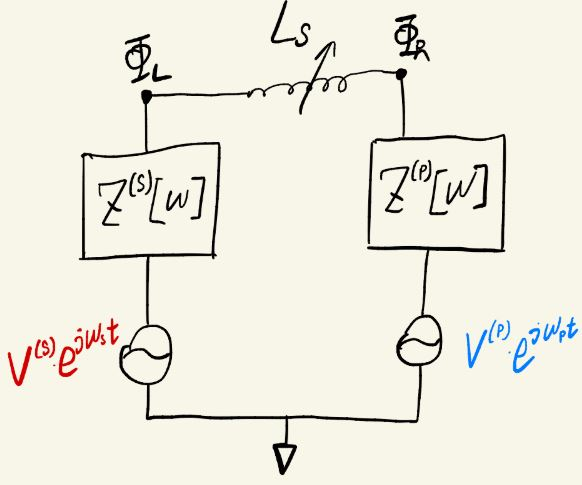
\includegraphics[width=7cm]{figures/circuit_2}
% % \caption
% % {\label{fig:circuit_2} Thevenin equivalent circuit}
% % \end{figure}

% (Note that the relation between Thevenin voltage source $V^{(s/p)}$ and actual voltage at end of transmission line has to be simulated as well. )

% For resonance parametric amplification, besides the pumpistor (acting like a negative resistance), we also need a mode around signal frequency. This section discusses how to guarantee a mode with well-defined frequency and SNAIL participation when designing external coupling network. 

% When talking about resonance condition, let's first keep only the linear part of \eq{eq:It}: 

% \begin{equation}\label{eq:LJ}
% I(t) = I_c c_2 \tilde{\varphi} = 
% \frac{\Phi_L(t) - \Phi_R(t) }{L_J} - M\phi_0\varphi_\min/L_J
% \end{equation}

Outgoing wave solution: 
(argue that a discrete set)


There's a discrete set of ${\omega_k}$ that satisfies $j \Im Z_E[\omega_k] + j L_J \omega_k = 0$

We assume that the near-resonance response can be well-characterized by a LCR circuit. 

We should have: 
\begin{equation}\label{eq:m}
m:= \frac{\Im Z_E'[\omega_a]}{L_J} = \frac{2L - L_J}{L_J}
\end{equation}

participation ratio: 
\begin{equation}
p:= \frac{L_J}{L} = \frac{2}{m + 1}
\end{equation}



Pump frequency: $\omega_p = 2 (\omega_a + \Delta)$

Signal frequency: $\omega_s = \omega_p/2 + \omega = \omega_a + \Delta + \omega$

Idler frequency: $\omega_i = \omega_p - \omega_s = \omega_a + \Delta - \omega$

\begin{equation}\label{eq:ZE}
Z_E[\omega_s]= \frac{\kappa_a}{2}L_J - j \omega_a L_J + j m L_J (\omega_s - \omega_a)
\end{equation}


Specifically, we want the SPA mode linewidth $\kappa_a$ to be dominated by signal port coupling.
i.e. $\Re Z^{(s)}[\omega_a]= \frac{\kappa_a}{2}L_J$, $\Re Z^{(p)}[\omega_a] \approx 0$

In this case, assuming both signal and idler are near resonance, \eq{eq:ZJ} can be written as: 
\begin{equation}\label{eq:ZJ'}
\begin{aligned}
	Z_J[\omega_s] &= \frac{j L_J \omega_s }{1 - \frac{\abs{\epsilon}^2}{1 - jL_J \omega_i/Z_E^*[\omega_i]}}\\
	&= \frac{j L_J (\omega_a + \Delta + \omega) \left[ \frac{\kappa_a}{2} - j \frac{2}{p}(\Delta - \omega)\right]}{(1-\abs{\epsilon}^2)\left[ \frac{\kappa_a}{2} - j \frac{2}{p}(\Delta - \omega)\right] - j \abs{\epsilon}^2 (\omega_a + \Delta - \omega)}
\end{aligned}
\end{equation}




To do: 

......

At the same time, the signal port network can be characterized by input impedance $Z^{(s)}$ (with the other port 50 $\Omega$ loaded), resulting in linear response between current $I$ and node voltage $V_L = \dot{\Phi}_L$: 
\begin{equation}\label{eq:LL}
	V_L(t) = - \integral{Z^{(s)}(t-\tau) I(\tau)}{\tau}{}{}
\end{equation}
and similarly for the right hand side: 
\begin{equation}\label{eq:RR}
	V_R(t) = \integral{Z^{(p)}(t-\tau) I(\tau)}{\tau}{}{}
\end{equation}

Laplace transform on \eq{eq:LL} and \ref{eq:RR}, as well as \eq{eq:LJ}, we get: 
\begin{equation}\label{eq:Is}
\begin{aligned}
I[s] &= \frac{\Phi_L[s] - \Phi_R[s] }{L_J}\\
-s \Phi_L[s] &= Z^{(s)}[s] I[s] \\
s \Phi_R[s] &= Z^{(p)}[s] I[s]
\end{aligned}
\end{equation}

or written equivalently:

\begin{equation}
\(
\begin{matrix}
1 & \frac{s}{Z^{(s)}} & 0 \\
1 & 0 & -\frac{s}{Z^{(p)}} \\
1 & -1/L_J & 1/L_J
\end{matrix}
\)	
\(
\begin{matrix}
I\\
\Phi_L\\
\Phi_R
\end{matrix}
\)
 = 0
\end{equation}

Existance of non-trivial solutions requires: 
\begin{equation}
	Z^{(s)}[s] + Z^{(p)}[s] =  - s L_J
\end{equation}

If we write $s = - \kappa_a/2 + j \omega$: 
\begin{align}
	\Im{Z^{(s)}[-\kappa_a/2 + j \omega]} + \Im{Z^{(p)}[-\kappa_a/2 + j \omega]} &=  - \omega L_J \label{eq:R1}\\
	\Re{Z^{(s)}[-\kappa_a/2 + j \omega]} + \Re{Z^{(p)}[-\kappa_a/2 + j \omega]} &=  \frac{\kappa_a}{2} L_J  \label{eq:R2}
\end{align}
Assuming a set of $\{\omega_k\}$ and $\{\kappa_k\}$ that satisfy these conditions, solution to the system will be in the form of linear combination of eigenmodes: 
\begin{equation}
	I(t) = \sum_k I_{\omega_k} \exp{- \frac{\kappa_k}{2} t} \exp{j\omega_k t}
\end{equation}
with $\omega_k$ being frequency of the k-th eigenmode, and $\kappa_k/2$ being amplitude damping rate of that mode. 

To design an SPA mode with arbitrary coupling networks, imaginary (reactive) parts of input impedance $Z^{(s)}$ and $Z^{(p)}$ has to satisfy requirement \ref{eq:R1} at desired mode frequency $\omega_a$. And reasonable $\kappa_a$ for this mode has to be achieved by real part of $Z^{(s)}$ (since $\Re{Z^{(p)}}$ should be close to 0 to prevent signal leakage from pump port). Note that SNAIL expansion parameter $c_2$ is dependent on external flux bias. As $L_J$ varies with flux, so does the $\omega$ that satisfies \eq{eq:R1}, thus tunes the mode frequency. For degenerate amplification, no other modes should exist within the frequency range of interest. 

(Extract SNAIL inductance participation from slope of imaginary part of input impedance)

We can always get \textbf{energy participation} of a component from field simulation. And what we usually do is assuming the SNAIL is a lumped inductive element (no E field energy stored in it), then \textbf{inductance participation} is always twice the energy perticipation. 

Here I propose an easier way to do so by extracting SNAIL \textbf{inductance participation} in the mode, which lay a requirement for the input impedances "apriori" before a full field simulation. This would be easier than "run HFSS and change paramters" especially when we want to optimize multiple things iteratively. 

We can generally define total admittance of the loop $Y_\sys[\omega] = \(Z^{(s)}[\omega] + Z^{(p)}[\omega] + j \omega L_J\)^{-1}$. 

An assumption I make is that behaviour of $Y_\sys[\omega]$ near $\omega_a$ (for whatever frequency my signal could lie) can be modeled for by a simple RLC. (This assumption is much weaker than Foster theorem: I'm only talking about one mode.)

% \begin{figure}[htb]
% 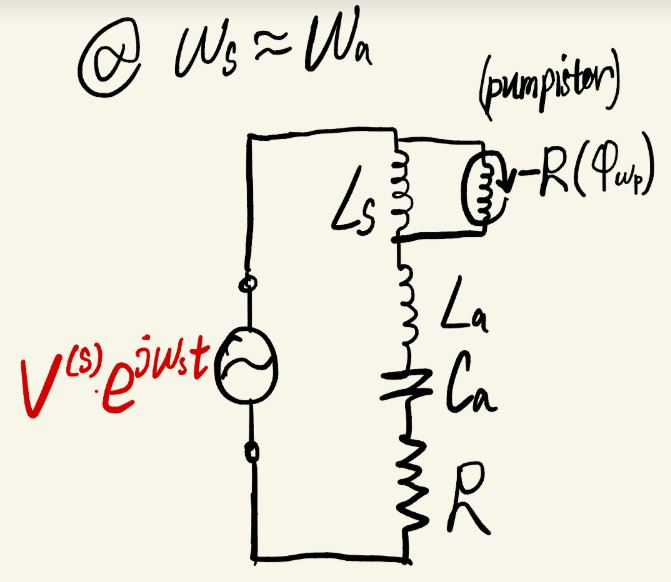
\includegraphics[width=6.5cm]{figures/circuit_3}
% \caption
% {\label{fig:circuit_3} Approximate circuit at $\omega_s \approx \omega_a$}
% \end{figure}

The signal Thevenin voltage source $V^{(s)}$ sees the whole system as $Y_\sys[\omega_s]$, that responds exactly the same (for near resonance $\omega_s$) as a series RLC. 

The RLC model should account for the mode frequency $\omega_a$, residual of $\Im{Y_\sys}$ at $\omega_a$, and energy damping rate $\kappa_a$ of the mode. (To account for amplification, we should put a pumpistor in parallel with $L_J$.) 

\par
\par
**How this model helps: 

Using this model, we can calculate equivalent $L_a$ and $C_a$ from the values and slopes of imaginary part of the two input impedances (from linear simulation). 
All later nonlinearity calculation can be easily done analytically, and all existing results from mode amplitude $a$ and $\ad$ language applies directly. 
Doesn't involve the simulated $Z[\omega]$ function in calculation, and doesn't need harmonic balance simulation. 

Note that 4-th and higher orders nonlinearity calculated from this circuit are different from Foster circuit BBQ. Following the current conservation argument in Appendix A of \cite{SPA}, we have to treat the nonlinear inductance in series with linear inductance, unlike in Foster circuit BBQ where nonlinearity is treated in parallel with linear part. Another way to interprate the reason why Foster BBQ break down for SPA is that SNAIL participation in higher modes are non-negligible, therefore renormalization from higher modes has to be accounted for. 



\section{Evaluate SPA reflection}\label{appen:S11}

Recall that the reflection and transmission coefficients (in S-matrix) for a lumped impedance $Z_J$ is: 
\[
R = \frac{Z_J}{Z_J+2 Z_c} \qquad
T = \frac{2Z_c}{Z_J+2 Z_c}
\]
As the effective impedance for a pumped SNAIL array is derived in \eq{eq:ZJ}, it applies directly into the concatenated SPA: 

\begin{equation}
V_0 = \frac{S^{(s)}_{21} V_s}{1 - \( R + \frac{S^{(p)}_{11} T^2}{1- S^{(p)}_{11} R } \) S^{(s)}_{22}} 
\end{equation}



Overall reflection coefficient of the SPA is given by: 
\begin{equation}\label{eq:S11}
\frac{V_\out}{V_\in} = S^{(s)}_{11} + \frac{S^{(s)}_{21} S^{(s)}_{12} \Gamma }{1 - \Gamma S^{(s)}_{22}} 
\end{equation}
where we name:
\begin{equation}\label{eq:Gamma}
\begin{aligned}
\Gamma &=  R + \frac{S^{(p)}_{11} T^2}{1- S^{(p)}_{11} R } \\
&= \frac{Z_J}{Z_J+2 Z_c} + \frac{  \frac{Z^{(p)}-Z_c}{Z^{(p)}+Z_c} \( \frac{2Z_c}{Z_J+2 Z_c} \)^2}{1-\frac{Z^{(p)}-Z_c}{Z^{(p)}+Z_c} \frac{Z_J}{Z_J+2 Z_c}}\\
&=\frac{1}{Z_J + 2Z_c} \( Z_J + \frac{2Z_c}{\frac{Z_J+2Z_c}{Z^{(p)} -Z_c}+1} \)\\
&= \frac{Z_J + Z^{(p)} - Z_c}{Z_J + Z^{(p)} + Z_c}
\end{aligned}
\end{equation}
in which we have introduced pump port output impedance (seen by the SNAIL array): 
\[
Z^{(p)} = Z_c \frac{1 + S^{(p)}_{11}}{1- S^{(p)}_{11}}
\]
Similarly, signal port output impedance (seen by the SNAIL array) should be: 
\[
Z^{(s)} = Z_c \frac{1 + S^{(s)}_{22}}{1- S^{(s)}_{22}}
\]

In that case, the total external impedance $Z_E[\omega]$ seen by the SNAIL array which appears in \eq{eq:ZS} would compose of: 
\begin{equation}
Z_E = Z^{(s)} + Z^{(p)}
\end{equation}

And \eq{eq:S11} is equivalent to: 
\begin{equation}\label{eq:S11'}
\begin{aligned}
\frac{V_\out}{V_\in} &= S^{(s)}_{11} + {S^{(s)}_{21}}{S^{(s)}_{12}} \frac{(Z^{(s)} + Z_c)(Z_J + Z^{(p)} - Z_c)}{2Z_c(Z_J + Z^{(s)} + Z^{(p)})} \\
&= S^{(s)}_{11} + {S^{(s)}_{21}}{S^{(s)}_{12}} \frac{Z^{(s)} + Z_c}{2Z_c} \( 1 - \frac{Z^{(s)} + Z_c}{Z_J + Z_E}\)
\end{aligned}
\end{equation}

Such a signal port filter network should be reciprocal: $S^{(s)}_{12} = S^{(s)}_{21}$ and unitary: $S^{(s)\dagger} S^{(s)} = I$ (assuming lossless). 

After some math, we have $S^{(s)}_{11}S^{(s)}_{22} - S^{(s)2}_{21} = \exp{j \theta}$ where $S^{(s)}_{11} = \exp{j \theta} S^{(s)*}_{22}$

% $\abs{S^{(s)}_{11}}^2 + \abs{S^{(s)}_{21}}^2 = \abs{S^{(s)}_{21}}^2 + \abs{S^{(s)}_{22}}^2 = 1$

Plug into \eq{eq:S11'}: 
\begin{equation*}
\begin{aligned}
\frac{V_\out}{V_\in} &= \exp{j \theta} S^{(s)*}_{22} + \exp{j \theta} \(\abs{S^{(s)}_{22}}^2 - 1\)
\frac{Z^{(s)} + Z_c}{2Z_c} \( 1 - \frac{Z^{(s)} + Z_c}{Z_J + Z_E} \) \\
&= \exp{j \theta} \left[ 
\frac{Z^{(s)*} - Z_c}{Z^{(s)*} + Z_c} + 
\(
\abs{\frac{Z^{(s)} - Z_c}{Z^{(s)} + Z_c}}^2 - 1
\)
\frac{Z^{(s)} + Z_c}{2Z_c} \( 1 - \frac{Z^{(s)} + Z_c}{Z_J + Z_E} \)
\right]\\
&= \exp{j \theta} \left[ 
\frac{Z^{(s)*} - Z_c}{Z^{(s)*} + Z_c} + 
\(
\frac{\abs{Z^{(s)} - Z_c}^2 - \abs{Z^{(s)} + Z_c}^2}{(Z^{(s)} + Z_c)(Z^{(s)*} + Z_c)}
\)
\frac{Z^{(s)} + Z_c}{2Z_c} \( 1 - \frac{Z^{(s)} + Z_c}{Z_J + Z_E} \)
\right]\\
&= \frac{\exp{j \theta}}{Z^{(s)*} + Z_c} \left[ 
Z^{(s)*} - Z_c + 
\frac{-4 \Re Z^{(s)} Z_c}{2Z_c}
\( 1 - \frac{Z^{(s)} + Z_c}{Z_J + Z_E} \)
\right] \\
&= \frac{\exp{j \theta}}{Z^{(s)*} + Z_c} \left[ 
Z^{(s)*} - 2\Re Z^{(s)} - Z_c + 2 \Re Z^{(s)}
\frac{Z^{(s)} + Z_c}{Z_J + Z_E}
\right] \\
&= \exp{j \theta}\frac{Z^{(s)} + Z_c}{Z^{(s)*} + Z_c} 
\(\frac{2\Re Z^{(s)}}{Z_J + Z_E} - 1 \)
\end{aligned}
\end{equation*}

So if we look at power gain $G[\omega] = \abs{\frac{V_\out[\omega]}{V_\in[\omega]}}^2$: 
\begin{equation}
\begin{aligned}
G[\omega_s] &=  
\abs{\frac{2\Re Z^{(s)}[\omega_s]}{Z_J[\omega_s] + Z_E[\omega_s]} - 1}^2\\
&= \abs{ \frac{\kappa_a}{\frac{Z_J[\omega_s]}{L_J} + \frac{\kappa_a}{2} - j (\omega_a - m (\Delta + \omega))} - 1 }^2
\end{aligned}
\end{equation}

Recall that: 
\[
Z_J[\omega_s] = \frac{j L_J (\omega_a + \Delta + \omega) \left[ \frac{\kappa_a}{2} - j \frac{2}{p}(\Delta - \omega)\right]}{(1-\abs{\epsilon}^2)\left[ \frac{\kappa_a}{2} - j \frac{2}{p}(\Delta - \omega)\right] - j \abs{\epsilon}^2 (\omega_a + \Delta - \omega)}
\]

Specifically, $Z_J[\omega_s] = j L_J (\omega_a + \Delta + \omega)$ without pump (i.e. when $\epsilon = 0$). In this case: 

\begin{equation}
\begin{aligned}
\frac{V_\out[\omega_s]}{V_\in[\omega_s]} &= \exp{j \theta}\frac{Z^{(s)}[\omega_s] + Z_c}{Z^{(s)*}[\omega_s] + Z_c} 
\(\frac{\kappa_a}{\frac{\kappa_a}{2} + j\frac{2}{p} (\omega_s - \omega_a)} - 1 \)\\ 
&= \exp{j (\theta + 2\theta_{\omega_s})}
\frac{\frac{p}{2}\frac{\kappa_a}{2} + j(\omega_s - \omega_a)}{\frac{p}{2}\frac{\kappa_a}{2} - j(\omega_s - \omega_a)}
\end{aligned}
\end{equation}
Here $\theta_{\omega_s}$ is phase factor of $\Re Z^{(s)}[\omega_s] + Z_c + j \Im Z^{(s)}[\omega_s]$, which should be smooth over frequency. So we can take it as adding an overall slope on the phase roll. 



% \begin{equation*}
% \begin{aligned}
% Z_J[\omega_s] &= \frac{j L_J (\omega_a + \Delta + \omega) \left[ \frac{\kappa_a}{2} - j \frac{2}{p}(\Delta - \omega)\right]}{(1-\abs{\epsilon}^2)\left[ \frac{\kappa_a}{2} - j \frac{2}{p}(\Delta - \omega)\right] - j \abs{\epsilon}^2 (\omega_a + \Delta - \omega)} \\
% & \approx \frac{L_J(\omega_a + \Delta + \omega)}{-\abs{\epsilon}^2} \frac{(m+1)(\Delta - \omega) + j\frac{\kappa_a}{2}}{\frac{\kappa_a}{2} + j(\omega_a - m(\Delta - \omega))}
% \end{aligned}
% \end{equation*}

% \[
% -\frac{\abs{\epsilon}^2}{\omega_a + \Delta + \omega} \frac{Z_J[\omega_s]}{L_J} = 
% \frac{\frac{\kappa_a}{2}(\omega_a + \Delta - \omega)}{\abs{\frac{\kappa_a}{2} + j(\omega_a - m(\Delta - \omega))}^2} + j \left[1 - \frac{(\omega_a + \Delta - \omega)(\omega_a - m (\Delta - \omega) )}{\abs{\frac{\kappa_a}{2} + j(\omega_a - m(\Delta - \omega))}^2}  \right] 
% \]

% Name $G[\omega_s] = \abs{ \frac{\kappa_a - A}{A} }^2 $, where: 

% \[
% \Re A = \frac{\kappa_a}{2} -  \frac{\omega_a + \Delta + \omega}{\abs{\epsilon}^2} \frac{\frac{\kappa_a}{2}(\omega_a + \Delta - \omega)}{\abs{\frac{\kappa_a}{2} + j(\omega_a - m(\Delta - \omega))}^2} 
% \]

% \[
% \Im A = -(\omega_a - m (\Delta + \omega)) -  \frac{\omega_a + \Delta + \omega}{\abs{\epsilon}^2} \left[1 - \frac{(\omega_a + \Delta - \omega)(\omega_a - m (\Delta - \omega) )}{\abs{\frac{\kappa_a}{2} + j(\omega_a - m(\Delta - \omega))}^2}  \right] 
% \]

% Therefore: 
% \[
% G[\omega_s] = 1 + \frac{\kappa_a^2 B}{(\Re A)^2 + (\Im A)^2}
% \]
% where we have named:
% \begin{equation*}
% \begin{aligned}
% B &= \frac{ \frac{1}{\abs{\epsilon}^2} (\omega_a + \Delta + \omega)(\omega_a + \Delta - \omega)}{\abs{\frac{\kappa_a}{2} + j(\omega_a - m(\Delta - \omega))}^2} \\
% &= \frac{ \frac{1}{\abs{\epsilon}^2}  ((\omega_a + \Delta)^2 - \omega^2)}{ \frac{\kappa_a^2}{4} + (\omega_a - m(\Delta - \omega))^2} \\
% & \approx \frac{1}{\abs{\epsilon}^2}
% \(
% 1 + 2(m+1) \frac{\Delta}{\omega_a} - 2m \frac{\omega}{\omega_a}
% \)
% \end{aligned}
% \end{equation*}


% \[
% (\Re A)^2 = \frac{\kappa_a^2}{4} (1-B)^2
% \]



% \begin{equation*}
% \begin{aligned}
% -\Im A &= \omega_a - m (\Delta + \omega) +  \frac{\omega_a + \Delta + \omega}{\abs{\epsilon}^2}  - (\omega_a - m (\Delta - \omega) )B\\
% &= 
% \omega_a \(1 + \frac{1}{\abs{\epsilon}^2}-B\) + 
% \Delta \(-m + \frac{1}{\abs{\epsilon}^2} + mB\) + 
% \omega \(-m + \frac{1}{\abs{\epsilon}^2} - mB\)
% \\
% & \approx \omega_a - m(\Delta + \omega) - \frac{m+1}{\abs{\epsilon}^2}(\Delta - \omega)
% \end{aligned}
% \end{equation*}


% \[
% (\Im A)^2 = 
% \(
% \omega_a - m(\Delta + \omega) - \frac{2}{p\abs{\epsilon}^2}(\Delta - \omega)
% \)^2
% \]



\begin{equation}
G = 1 + \frac{\kappa_a^2 \abs{\epsilon}^2 [(\omega_a + \Delta)^2 - \omega^2]}{(1+m -m \abs{\epsilon}^2)^2\kappa_a^2\omega^2 + 
\(\frac{\kappa_a^2}{4}(1-\abs{\epsilon}^2) + \Delta^2 (1+2m+m^2 (1-\abs{\epsilon}^2) )  - \omega^2 (1+2m+m^2 (1-\abs{\epsilon}^2) ) + 2m\abs{\epsilon}^2 \Delta \omega_a - \abs{\epsilon}^2 \omega_a^2
\)^2}
\end{equation}


\begin{equation}
G = 1 + \frac{\kappa_a^2 \abs{\epsilon}^2 [(\omega_a + \Delta)^2 - \omega^2]}{(1+m)^2\kappa_a^2\omega^2 + 
\(\frac{\kappa_a^2}{4} + \Delta^2 (1+m)^2  - \omega^2 (1+m)^2 + 2m\abs{\epsilon}^2 \Delta \omega_a - \abs{\epsilon}^2 \omega_a^2
\)^2}
\end{equation}

\begin{equation}
G = 1 + \frac{\kappa^2 \abs{\epsilon' \omega_p/2}^2 }{\kappa^2\omega^2 + 
\(\frac{\kappa^2}{4} + \Delta^2 - \omega^2 - \abs{\epsilon' \omega_p/2}^2
\)^2}
\end{equation}



When signal detuning $\omega \approx 0$: 
\begin{equation}
G = 1 + \frac{\kappa^2 \abs{\epsilon' \omega_p/2}^2 }{
\(\frac{\kappa^2}{4} + \Delta^2 - \abs{\epsilon' \omega_p/2}^2
\)^2}
\end{equation}

where $\epsilon' = \frac{\epsilon}{1+m} = \frac{p c_3\varphi_{\omega_p}}{4c_2}$, $\kappa = \frac{p}{2}\kappa_a$

\section{Verification: A lumped SPA}

Impedance seen by the SNAIL: 

\begin{equation*}
Z_E[\omega] = \frac{R}{1 + j \omega RC} + j \omega L
\end{equation*}

We can evaluate its real and imaginary part respectively:
\begin{equation*}
\begin{aligned}
\Re Z_E[\omega] &= \frac{R}{1 + \omega^2 R^2C^2} \\
& \approx \frac{1}{\omega^2 R C^2} \(1- \frac{1}{\omega^2 R^2 C^2}\) \\
& \approx \frac{1}{\omega_a^2 R C^2} \( 1 - \frac{2\Delta}{\omega_a} \) \(1- \frac{1}{\omega_a^2 R^2 C^2}\) \\
&= \frac{L_J + L}{R C} \( 1 - \frac{2\Delta}{\omega_a} \) \(1- \frac{Z_a^2}{R^2}\)
\end{aligned}
\end{equation*}

\begin{equation*}
\begin{aligned}
\Im Z_E[\omega] &= \omega L - \frac{\omega R^2 C}{1 + \omega^2 R^2C^2} \\
& \approx \omega \(L - \frac{1}{\omega^2 C} \(1- \frac{Z_a^2}{R^2}\) \) \\
& \approx (\omega_a + \Delta) \(L - (L_J + L) \(1- \frac{2\Delta}{\omega_a} \) \) \\
&= -\omega_a L_J + L_J \(\frac{2L}{L_J}+1\)\Delta
\end{aligned}
\end{equation*}

According to the relations in Section \ref{appen:mode}

\begin{equation*}
\Im Z_E[\omega_a] = -\omega_a L_J
\end{equation*}

\begin{equation*}
m = \frac{\Im Z_E[\omega_a]}{L_J} = \frac{2L}{L_J} + 1
\end{equation*}

And we see that SNAIL participation ratio is: 

\begin{equation*}
p = \frac{2}{m+1} = \frac{L_J}{L + L_J}
\end{equation*}

\begin{equation*}
\kappa = \frac{p}{2} \kappa_a = \frac{L_J}{2(L + L_J)} \frac{2 \Re Z_E[\omega_a]}{L_J} = \frac{1}{RC}
\end{equation*}



\section{Include Kerr into pumpistor model}

\begin{equation*}
I(t) = \frac{E_j}{\phi_0} \( c_2\tilde{\varphi} +  \frac{c_3}{2} \tilde{\varphi}^2  + \frac{c_4}{6} \tilde{\varphi}^3 + \cdots \)
\end{equation*}

\begin{equation*}
\begin{aligned}
	\tilde{\varphi}(t) &= \Re \( \varphi_{\omega_s} \exp{j\omega_s t} + \varphi_{\omega_p} \exp{j\omega_p t} + \varphi^*_{\omega_i} \exp{-j\omega_i t} \) \\
	&= \frac{1}{2} \( \varphi_{\omega_s} \exp{j\omega_s t} + \varphi_{\omega_p} \exp{j\omega_p t} + \varphi^*_{\omega_i} \exp{-j\omega_i t} + 
	\varphi^*_{\omega_s} \exp{-j\omega_s t} + \varphi^*_{\omega_p} \exp{-j\omega_p t} + \varphi_{\omega_i} \exp{j\omega_i t}
	 \)
\end{aligned}
\end{equation*}

\begin{equation*}
\begin{aligned}
	I(t) &= \Re \( I_{\omega_s} \exp{j\omega_s t} + I_{\omega_p} \exp{j\omega_p t} + I^*_{\omega_i} \exp{-j\omega_i t} \) \\
	&= \frac{1}{2} \( I_{\omega_s} \exp{j\omega_s t} + I_{\omega_p} \exp{j\omega_p t} + I^*_{\omega_i} \exp{-j\omega_i t} + I^*_{\omega_s} \exp{-j\omega_s t} + I^*_{\omega_p} \exp{-j\omega_p t} + I_{\omega_i} \exp{j\omega_i t}
	 \)
\end{aligned}
\end{equation*}


\begin{equation}
	I_{\omega_s} = I_c \(c_2 \varphi_{\omega_s} + \frac{c_3}{2} \varphi_{\omega_p} \varphi^*_{\omega_i} + \frac{c_4}{8} \( |\varphi_{\omega_s}|^2 +  2|\varphi_{\omega_i}|^2 + 2|\varphi_{\omega_p}|^2\) \varphi_{\omega_s}\) 
\end{equation}

\begin{equation}
Y_S[\omega_s] = \frac{c_2}{j\omega_s ML_J}\(1 + \frac{c_4}{8c_2}\( |\varphi_{\omega_s}|^2 +  2|\varphi_{\omega_i}|^2 + 2|\varphi_{\omega_p}|^2\) \) + \frac{\frac{c_3}{2} \frac{\varphi_{\omega_p} \varphi^*_{\omega_i}}{\varphi_{\omega_s}}}{j\omega_s ML_J}
\end{equation}


\begin{equation}
\(
\begin{matrix}
I_{\omega_s}\\
I^*_{\omega_i}
\end{matrix}
\)
= 
\frac{1}{j L_J}
\(
\begin{matrix}
\frac{1 + \delta_s}{\omega_s} & \frac{-\epsilon}{\omega_i}\\
\frac{-\epsilon^*}{\omega_s} & \frac{1 + \delta_i}{\omega_i}
\end{matrix}
\)
\(
\begin{matrix}
V_{\omega_s}\\
V^*_{\omega_i}
\end{matrix}
\)
\end{equation}




To get the 2nd order perturbation correction (current conservation analysis): 

need also to include the higher idler frequency $\omega_h = \omega_s + \omega_p = 2\omega_p - \omega_i $


\begin{equation}
	I_{\omega_s} = I_c \(c_2 \varphi_{\omega_s} + \frac{c_3}{2} \( \varphi_{\omega_p} \varphi^*_{\omega_i} + \varphi^*_{\omega_p} \varphi_{\omega_h}\) + \frac{c_4}{4} |\varphi_{\omega_p}|^2 \varphi_{\omega_s}\) 
\end{equation}


Let's consider the Kerr effect due to pump only, and denote: 
\begin{equation}
\delta = \frac{c_4}{4c_2}|\varphi_{\omega_p}|^2
\end{equation}

We get: 

\begin{equation}
\(
\begin{matrix}
I_{\omega_s}\\
I^*_{\omega_i}\\
I_{\omega_h}
\end{matrix}
\)
= 
\frac{1}{j L_J}
\(
\begin{matrix}
\frac{1 + \delta}{\omega_s} & \frac{-\epsilon}{\omega_i} & \frac{\epsilon^*}{\omega_h}\\
\frac{-\epsilon^*}{\omega_s} & \frac{1 + \delta}{\omega_i} & 0 \\
\frac{\epsilon}{\omega_s} & 0 & \frac{1 + \delta}{\omega_h}
\end{matrix}
\)
\(
\begin{matrix}
V_{\omega_s}\\
V^*_{\omega_i}\\
V_{\omega_h}
\end{matrix}
\)
\end{equation}

which should be put together with other linear elements in the circuit and solved self-consistently, i.e.





\begin{equation*}
\begin{aligned}
	I^*_{\omega_i} Z_E[-\omega_i] + V^*_{\omega_i} &= 0 \\
	I_{\omega_h} Z_E[\omega_h] + V_{\omega_h} &= 0
\end{aligned}
\end{equation*}

Consequently: 


\begin{equation*}
\begin{aligned}
	\frac{V^*_{\omega_i}}{V_{\omega_s}} &= \frac{\epsilon^*}{(1+\delta)\frac{\omega_s}{\omega_i} - \frac{j L_J \omega_s}{Z_E[-\omega_i]} } \\
	\frac{V_{\omega_h}}{V_{\omega_s}} &= \frac{-\epsilon}{(1+\delta)\frac{\omega_s}{\omega_h} + \frac{j L_J \omega_s}{Z_E[\omega_h]} }
\end{aligned}
\end{equation*}



So the full expression should be: 

\begin{equation}
	Z_J[\omega_s] = \frac{j L_J \omega_s }{1 + \delta - \frac{\abs{\epsilon}^2}{1 + \delta - jL_J \omega_i/Z_E^*[\omega_i]} - \frac{\abs{\epsilon}^2}{1 + \delta + jL_J \omega_i/Z_E[\omega_h]}}
\end{equation}



While let us neglect $Z_E[\omega_h]$ for now (assuming it's a short). Keeping up to 1st order in $\delta$ and $\abs{\epsilon}^2$: 

\begin{equation}
Z_J[\omega_s] = \frac{j L_J (\omega_a + \Delta + \omega) \left[ (1+\delta) \( \frac{\kappa_a}{2} - j \frac{2}{p}(\Delta - \omega) \) + j \delta (\omega_a + \Delta - \omega)\right]}{(1 + 2\delta -\abs{\epsilon}^2) \( \frac{\kappa_a}{2} - j \frac{2}{p}(\Delta - \omega)\) + j (\delta - \abs{\epsilon}^2) (\omega_a + \Delta - \omega)}
\end{equation}



\section{Impedance engineered broadband JPA}

We have already shown that the gain profile has a frequency (signal detuning from $\omega_p/2$) dependence: 
\begin{equation*}
G[\omega] \approx \frac{\kappa^2 \abs{\epsilon' \omega_p/2}^2 }{\kappa^2\omega^2 + 
\(\frac{\kappa^2}{4} + \Delta^2 - \omega^2 - \abs{\epsilon' \omega_p/2}^2
\)^2}
\end{equation*}

When using a JPA, we usually talk about its gain at the peak, i.e. at $\omega \approx 0$: 
\begin{equation*}
G_0 \approx \frac{\kappa^2 \abs{\epsilon' \omega_p/2}^2 }{
\(\frac{\kappa^2}{4} + \Delta^2 - \abs{\epsilon' \omega_p/2}^2
\)^2}
\end{equation*}

After some maths, we get: 
\begin{equation}
G[\omega] = \frac{G_0}{1 + (\omega/\Gamma)^2}
\end{equation}
where 
\begin{equation}\label{eq:GainBW}
\Gamma = \frac{1}{\sqrt{G_0}} \frac{\kappa \abs{\epsilon' \omega_p/2}}{\sqrt{2 \(\frac{\kappa^2}{4} - \Delta^2 + \abs{\epsilon' \omega_p/2}^2
\)}}
\end{equation}

Worth noting, in the case of zero pump detuning ($\Delta \approx 0$) and high gain ($\frac{\kappa^2}{4} + \Delta^2 - \abs{\epsilon' \omega_p/2}^2 \approx 0$), \eq{eq:GainBW} have a prettier looking: 

\begin{equation}\label{eq:GainBW}
2\Gamma = \frac{\kappa}{\sqrt{G_0}}
\end{equation}
i.e. FWHM in gain profile is approximately resonance linewidth $\kappa$ over root gain. This is the famous gain-bandwidth tradeoff. 



According to literature, engineering a slope in the real part of output impedance could made a broadband JPA beyond the gain-bandwidth tradeoff. 

As a reminder, previously in \eq{eq:ZE} we're assuming the real part of output impedance being constant around $\omega_a$ (i.e. the slope being negligible). 

Now we want to include the 

\begin{equation}
Z_E[\omega_s]= \frac{\kappa_a}{2}L_J + r L_J (\omega_s - \omega_a) - j \omega_a L_J + j m L_J (\omega_s - \omega_a)
\end{equation}

where we're assuming $\Re Z^{(p)}[\omega_a] = \Re Z^{(p)'}[\omega_a] = 0$ and: 
\begin{equation}\label{eq:r}
r:= \frac{\Re Z^{(s)'}[\omega_a]}{L_J}
\end{equation}


In this case: 
\begin{equation}
\begin{aligned}
G[\omega_s] &=  
\abs{\frac{2\Re Z^{(s)}[\omega_s]}{Z_J[\omega_s] + Z_E[\omega_s]} - 1}^2\\
&= \abs{ \frac{\kappa_a + 2r (\Delta + \omega)}{\frac{Z_J[\omega_s]}{L_J} + \frac{\kappa_a}{2} + r(\Delta + \omega) - j (\omega_a - m (\Delta + \omega))} - 1 }^2
\end{aligned}
\end{equation}

And
\begin{equation}
	Z_J[\omega_s] = \frac{j L_J (\omega_a + \Delta + \omega) \left[ \frac{\kappa_a}{2} + r(\Delta - \omega) - j \frac{2}{p}(\Delta - \omega)\right]}{(1-\abs{\epsilon}^2)\left[ \frac{\kappa_a}{2} + r(\Delta - \omega) - j \frac{2}{p}(\Delta - \omega)\right] - j \abs{\epsilon}^2 (\omega_a + \Delta - \omega)}
\end{equation}

Like what we did in section \ref{appen:S11}, let's start with the case of no pump: $Z_J[\omega_s] = j L_J \omega_s$ 

\begin{equation}
\begin{aligned}
\frac{V_\out[\omega_s]}{V_\in[\omega_s]} &= \exp{j \theta}\frac{Z^{(s)}[\omega_s] + Z_c}{Z^{(s)*}[\omega_s] + Z_c} 
\(\frac{\kappa_a + 2r(\omega_s - \omega_a) }{\frac{\kappa_a}{2} + r(\omega_s - \omega_a) + j(m+1)(\omega_s - \omega_a)} - 1 \)\\ 
&= \exp{j (\theta + 2\theta_{\omega_s})}
\frac{\frac{p}{2}\(\frac{\kappa_a}{2} + r(\omega_s - \omega_a)\) + j(\omega_s - \omega_a)}{\frac{p}{2} \(\frac{\kappa_a}{2} + r(\omega_s - \omega_a)\) - j(\omega_s - \omega_a)}
\end{aligned}
\end{equation}



\begin{equation}
G = 1 + \frac{ (\kappa_a + 2 r (\Delta + \omega)) (\kappa_a + 2 r (\Delta - \omega)) \abs{\epsilon}^2 [(\omega_a + \Delta)^2 - \omega^2]}{ \omega^2 \( (1+m)\kappa_a - 2r \abs{\epsilon}^2 \omega_a \)^2 +
\(\frac{\kappa_a^2}{4} + \Delta^2 (1+m)^2  - \omega^2 (1+m)^2 - \abs{\epsilon}^2 \omega_a^2 + r^2 (\Delta^2 - \omega^2) + r \Delta \kappa_a
\)^2}
\end{equation}


\begin{equation}
G = 1 + \frac{ \(\kappa'^2 - (p\omega/2)^2 \)\abs{\epsilon' \omega_p/2}^2}{ \omega^2  (\kappa^2 - 4r \kappa \abs{\epsilon'}^2 \omega_a) +
\( \frac{\kappa'^2}{4} + \Delta^2 - (1+r^2) \omega^2 - \abs{\epsilon' \omega_p/2}^2) 
\)^2}
\end{equation}

where $\kappa' = \kappa + p r \Delta = \frac{\kappa_a + 2r\Delta}{m+1}$


% \section{Calculation: two-port SPA pump leakage}\label{appen:leakage}

% ...... Easy part, just get the relation between $\varphi_{\omega_p}$ and $V^{(p)}$, calculate how much power at end of pump port transmission line gives $\varphi_{\omega_p}$ we need. 

% And convert (using signal port network simulation result) the current $I_{\omega_p}$ into power seen by signal port transmission line. 

% I've assumed stiff pump, which means I didn't do full harmonic balance. Which is doable though, by writing the \eq{eq:IV} like relation at $\omega_p$ also, and solving the three self-consistently. 
% (This will allow us to characterize pump depletion. But I personally don't want to do it this way. Filters have kind of complicated response over pump frequency range, and we'll have to use simulated $Z^{(p)}[\omega]$ in all calculations. That could result in less robustness in simulation result and larger deviation between simulation and experiment. Also, I think this is not directly related to the main point of this paper.)






% After getting $Z_\ZPF$ of the mode, we can quantize this mode and perform a strict QLE treatment to explain the coupling rate. 


% \begin{align}
% \dot{\Phi} &= \frac{Q}{C_a} \label{eq:Phidotdir} \\
% \dot{Q} &= -\frac{\Phi}{L_a} - \frac{1}{Z_C}(\dot{\Phi} - V_\in) \label{eq:Qdotdir}
% \end{align}
% where $V_\in(t)$ is drive voltage at the end of transimion line.

% Introducing annihilation/creation operator according to $\Phi = \Phi _\ZPF (a + \ad)$ and $Q =\ii Q_\ZPF (\ad - a)$, where:
% \begin{equation}
% \Phi_\ZPF = \sqrt{\frac{\hbar}{2} Z_\ZPF}, \qquad Q_\ZPF = \sqrt{\frac{\hbar}{2 Z_\ZPF}}
% \end{equation}

% and $Z_\ZPF = \sqrt{(L_J+L_a)/C_a}$. Then \eq{eq:Phidotdir} is equivalent to: 

% \begin{equation}\label{eq:a1}
% \dot{a} + \dot{a}^\dagger = \frac{\ii Q_\ZPF}{\Phi_\ZPF C_a} (\ad- a) = \ii \omega_a (\ad - a)
% \end{equation}





% We can decompose the Heisenberg picture operator $a(t)$ in Fourier space: 

% \begin{equation}\label{eq:aFT}
% a(t) = \frac{1}{2\pi} \integral{a[\omega] \exp{- \ii \omega t}}{\omega}{-\inf}{\inf}
% \end{equation}

% And \eq{eq:a1} in Fourier domain can be written as: 

% \begin{equation}\label{eq:a2}
% \ad[-\omega] = -\frac{\omega-\omega_a}{\omega+\omega_a} a[\omega]
% \end{equation}



% (Arbitrary coupling)

% Outgoing current from the system: 
% \begin{equation}
% \begin{aligned}
% I_\out(t) &= \frac{1}{2\pi}\integral{I_\out[\omega]\exp{j\omega t}}{\omega}{-\inf}{\inf} \\
% &= \frac{1}{2\pi}\integral{\left( j \omega \Phi_\ZPF (a[\omega] + \ad[-\omega]) - V_\in[\omega] \right) Y_\tot[\omega]\exp{j\omega t}}{\omega}{-\inf}{\inf}\\
% &= \frac{1}{2\pi}\integral{\left( j\frac{2\omega \omega_a}{\omega + \omega_a} \Phi_\ZPF a[\omega] - V_\in[\omega] \right) Y_\tot[\omega]\exp{j\omega t}}{\omega}{-\inf}{\inf}
% \end{aligned}
% \end{equation}


% The total admittance seen by the system is: 
% \begin{equation}\label{eq:Ytot}
% Y_\tot[\omega] = \frac{1}{Z[\omega]+Z_C}
% \end{equation}


% And the Quantum Langevin Equations under arbitrary coupling, which are the generalized case of $\eq{eq:Phidotdir}$ and $\eq{eq:Qdotdir}$, should be written as: 

% \begin{align}
% \dot{\Phi} &= \frac{Q}{C_a} \label{eq:Phidot} \\
% \dot{Q} &= -\frac{\Phi}{L_a} - I_\out(t) \label{eq:Qdot}\\
% I_\out[\omega] &= \left(j \omega \Phi[\omega] - V_\in[\omega]  \right) Y_\tot[\omega] \label{eq:Iout}
% \end{align}

% where we notice that the EOM of $\Phi$ doesn't change, so \eq{eq:a1} still stands. And \eq{eq:Qdot} can be written into: 

% \begin{equation}\label{eq:a3}
% \ii (\dot{a}^\dagger - \dot{a}) = -\omega_a (\ad + a) - \frac{1}{Q_\ZPF} I_\out
% \end{equation}


% Using \eq{eq:aFT} and \eq{eq:a2} we can obtain: 

% % \begin{equation}\label{eq:FT1}
% % \begin{aligned}
% % - \ii (\dot{a}^\dagger - \dot{a}) &= \frac{1}{2\pi}\integral{\left(\omega a[\omega] \exp{-\ii \omega t} + \omega a^\dagger[\omega] \exp{\ii \omega t}\right)}{\omega}{-\inf}{\inf} \\
% %   &= \frac{1}{2\pi}\integral{\omega ( a[\omega] - a^\dagger[- \omega] )\exp{- \ii \omega t}}{\omega}{-\inf}{\inf} \\
% %   &= \frac{1}{2\pi}\integral{ \frac{2\omega^2}{\omega + \omega_a} a[\omega] \exp{j \omega t}}{\omega}{-\inf}{\inf}
% % \end{aligned}
% % \end{equation}

% \begin{equation}
% \begin{aligned}
% \dot{a}^\dagger + \dot{a} &= \frac{1}{2\pi}\integral{\left(a[\omega] \exp{-\ii \omega t} + \ad[\omega] \exp{\ii \omega t}\right)}{\omega}{-\inf}{\inf} \\
% &= \frac{1}{2\pi}\integral{( a[\omega] + \ad[- \omega] )\exp{- \ii \omega t}}{\omega}{-\inf}{\inf} \\
% &= \frac{1}{2\pi}\integral{ \frac{2\omega_a}{\omega + \omega_a} a[\omega] \exp{j \omega t}}{\omega}{-\inf}{\inf}
% \end{aligned}
% \end{equation}


% And using \eq{eq:Iout}, we can write down the last term in \eq{eq:a3} from inverse-Fourier transform: 
% \begin{equation}
% \begin{aligned}
% I_\out(t) &= \frac{1}{2\pi}\integral{I_\out[\omega]\exp{j\omega t}}{\omega}{-\inf}{\inf} \\
% &= \frac{1}{2\pi}\integral{\left( j \omega \Phi_\ZPF (a[\omega] + \ad[-\omega]) - V_\in[\omega] \right) Y_\tot[\omega]\exp{j\omega t}}{\omega}{-\inf}{\inf}\\
% &= \frac{1}{2\pi}\integral{\left( j\frac{2\omega \omega_a}{\omega + \omega_a} \Phi_\ZPF a[\omega] - V_\in[\omega] \right) Y_\tot[\omega]\exp{j\omega t}}{\omega}{-\inf}{\inf}
% \end{aligned}
% \end{equation}


% Now we can finally rewrite the Quantum Langevin Equation \eq{eq:a3} in Fourier domain: 

% \begin{equation}
% \frac{2\omega^2}{\omega + \omega_a} a[\omega] =\frac{2\omega_a^2}{\omega + \omega_a}a[\omega] + \left( j\frac{2\omega \omega_a}{\omega + \omega_a} \Phi_\ZPF a[\omega] - V_\in[\omega] \right) \frac{Y_\tot[\omega]}{Q_\ZPF}
% \end{equation}

% \begin{equation}\label{eq:QLE}
% \left( \omega - \omega_a - j \frac{\omega \omega_a}{\omega + \omega_a} Z_\ZPF Y_\tot[\omega]\right) a[\omega] = - \frac{Y_\tot[\omega]}{2Q_\ZPF} V_\in[\omega]
% \end{equation}

% We can write \eq{eq:QLE} as: 
% \begin{equation}
% 	\left(\Delta[\omega] + \ii \frac{\kappa_a[\omega]}{2}\right)a[\omega] = -u[\omega]
% \end{equation}


% detuning: 
% \begin{equation}
% 	\Delta[\omega] = \omega - \omega_a - \frac{\omega \omega_a}{\omega + \omega_a} Z_\ZPF \Im Y_\tot[\omega]
% \end{equation}

% kappa for arbitrary coupling:
% \begin{equation}\label{eq:kappa}
% 	\kappa_a[\omega] = \frac{2 \omega_a \omega}{\omega_a + \omega} Z_\mathrm{ZPF} \Re Y_\tot[\omega]
% \end{equation}


% For an resonance mode $\omega_a = 1 / \sqrt{L_a C_a}$    ,    $Z_\mathrm{ZPF} = 1/\omega_a C_a$

% For direct coupling:$Y = 1/Z_C$ ,  $\kappa_a_d = 1/C_a Z_C$.

% For capacitive coupling: 
% \begin{equation}\label{eq:Y_c}
% Y_\tot[\omega] = \frac{1}{Z_C + \frac{1}{j \omega C_c}} \approx j \omega C_c (1-j \omega C_c Z_C)
% \end{equation}

% Therefore: 
% \begin{equation}\label{eq:kappa_c}
% \kappa_a_c = \frac{Z_C}{L_a}\frac{C_c^2}{C_a^2}=Z_C \omega_a^2\frac{C_c^2}{C_a}
% \end{equation}


\section{Noise}

\begin{equation*}
\begin{aligned}
\mathrm{NVR} &= P_{\mathrm{on}}/P_{\mathrm{off}}\\
&= \frac{G_\sys(T_\sys+G(T_Q+T_{\mathrm{add}}))}{G_\sys(T_\sys+T_Q)}\\
&= \frac{G}{T_\sys+T_Q}T_\mathrm{add} + \frac{T_\sys+G T_Q}{T_\sys+T_Q}
\end{aligned}
\end{equation*}





\end{document}